\lab{Python}{Data Structures}{Data Structures}
\label{lab:Python_DataStructures}
\objective{Empower students with basic knowledge of the fundamental, canonical data structures in order to understand performance and runtime characteristics.}

Both storing and retrieving data take time. As a data set grows, so too does the time required to manipulate it.
The overhead associated with working with large data sets makes it crucial that we have a fundamental knowledge of the data structures used to store them.
As we understand the characteristics of such data structures, we will be able to choose the data structure that will help us most efficiently access the data that we need.

\section*{Abstract Data Types}
The fundamental way to store data is via \emph{primitive data types}.
We are actually already quite familiar with these data types: booleans, strings, floats, and integers.
Most information that we care to store is in one of these forms; however, these primitive types can quickly become unwieldy for storing large amounts of information, especially since we rarely want to store a single string, float or integer. Rather, we want to organize our data in different ways depending on what we intend to do with it.
We can do this by using primitive data types, along with arrays, as our building blocks.
More complex data structures are called \emph{abstract data types}.
Typically, the performance of each abstract data type slows down as the size of the data structure increases.
However, some data structures slow down more slowly or gracefully than others.
This is why it is so important that we understand the underlying advantages and disadvantages of these structures.
Such an understanding allows us to choose the most optimal structure for our purposes.

Most abstract data types use an object called a \emph{node} to store data.
A node essentially acts as a box in which we store an arbitrary piece of data.
It usually serves as a building block for whichever kind of data structure we want to create; it is whatever we want it to be and it contains whatever we need it to contain.
This versatility lets us to define nodes to store absolutely anything; what they contain both depends on the data structure itself and data that is actually being stored.
Using nodes allows us to store extra information pertinent to the functioning of the datastructure.
For example, the node of a binary search tree (which we will later discuss in section \ref{Binary Search Tree}) contains three things: a piece of data, a reference to its left child, and a reference to its right child.
The node of a singly linked list contains only two things: a piece of data and a reference to the next node in the list.

\section*{Linked Lists}
\emph{Linked lists} are one of the most simple of all abstract data structures.
A linked list, in essence, is simply a list of nodes that are linked together.
There are two main types of linked lists: singly-linked (figure \ref{fig:singly_linked} and doubly-linked (figure \ref{fig:doubly_linked}.

\begin{figure}
\centering
\begin{tikzpicture}[->,>=stealth',shorten >=1pt,auto, node distance=1.5cm,thick,main node/.style={rectangle,draw}, minimum size=.5cm]
\tikzset{rect node/.style={rectangle, draw, minimum height = .5cm, minimum width=.2cm}}
  \node[main node] (1) {B};
  \node[main node] (2) [right of=1] {F};
  \node[main node] (3) [right of=2] {G};
  \node[main node] (4) [right of=3] {C};
  \node[draw = none, black!20!blue, node distance=1.5cm] [above left of=1](H) {Head};
\foreach \r in {1, 2, 3, 4}{
  \node[rect node][right of=\r, node distance = .36cm]{};}
\node[draw = none, node distance = 1.5cm] [right of=4]{};  % Centralize this particular figure
\foreach \s/\t  in {1/2, 2/3, 3/4}{
	\path[draw](\s) edge[shorten <=.1cm](\t);}
  \draw[black!20!blue] (H) edge (1.north);
\end{tikzpicture}
\caption{Singly-linked List}
\label{fig:singly_linked}
\end{figure}


A singly-linked node stores a piece of data (its value), and a single reference that points to the next node in the list.
Doubly-linked nodes have two references: one that points to the previous node and one that points to the next node in the list.
This allows for a doubly-linked list to be traversed in both directions, whereas a singly-linked list can only be traversed in one direction.
We begin to implement a singly-linked node class as follows:
\begin{lstlisting}
class Node(object):
    def __init__(self, data):
        self.next = None
        self.value = data
\end{lstlisting}

\begin{figure}
\centering
\begin{tikzpicture}[->,>=stealth',shorten >=1pt,auto, node distance=1.5cm, thick,main node/.style={rectangle,draw}, minimum size=.5cm]
\tikzset{rect node/.style={rectangle, draw, minimum height = .5cm, minimum width=.9cm}}
  \node[main node] (1) {B};
  \node[main node] (2) [right of=1] {F};
  \node[main node] (3) [right of=2] {G};
  \node[main node] (4) [right of=3] {C};
  \node[draw = none, black!20!blue, node distance = 1.5cm] [above right of=4] (T) {Tail};
  \node[draw = none, black!20!blue, node distance = 1.5cm] [above left of=1] (H) {Head};
  \node[rect node](1.5)[]{};
  \node[rect node](2.5)[right of=1.5]{};
  \node[rect node](3.5)[right of=2.5]{};
  \node[rect node](4.5)[right of=3.5]{};

\foreach \s/\t  in {1/2, 2/3, 2/1, 3/2, 3/4, 4/3}{
	\path[draw](\s) edge[shorten <=.1cm, shorten >=.1cm](\t);}	
  \draw[black!20!blue] (H) edge (1.north);
  \draw[black!20!blue] (T) edge (4.north);
\end{tikzpicture}
\caption{Doubly-linked List}
\label{fig:doubly_linked}
\end{figure}

We begin constructing a singly-linked list class with a reference to the head node:
\begin{lstlisting}
class SLinkedList(object):
    def __init__(self):
        self.head = None
\end{lstlisting}

Linked lists may also have a reference to the tail node and a size counter to keep track of the size of the list.
Including a tail reference allows us to avoid traversing the entire list each time we wish to insert at the end.
Similarly, without a size counter we would have to recount the list every time we wanted to know its size.
\begin{lstlisting}
class SLinkedList(object):
    def __init__(self):
        self.head = None
        self.tail = None
        self.size = 0

    def __len__(self):
        return self.size
\end{lstlisting}

\subsection*{Searching, Inserting and Removing}
To locate a node, our linked must start at the head of the list and follow references to other nodes until the desired node is found.
In a singly-linked list, it is also often a good idea to track the node prior to our index; this will prove useful for our insertion and removal methods.
We add a find method to our \li{SLinkedList} class:
\begin{lstlisting}
# Returns the node at the given index and the node previous to it.
def find(self, index):
    if index >= len(self):
        raise IndexError

    nfind = self.head
    nprev = None
    # Keeps track of the index of nfind.
    count = 0

    # Update nprev and nfind until we reach the node at the index desired.
    # nfind.next evaluates to True while nfind.next != None
    while count < index and nfind.next:
        count += 1
        nprev = nfind
        nfind = nfind.next
    return nprev, nfind
\end{lstlisting}

In order to insert or delete nodes found in the middle of the list, we must first locate the correct node by traversing the list, starting at the head and visiting each node.
Insertion itself is a very efficient procedure, but traversing the list to find the insert location takes longer as the size of the list grows.
However, because we already have head and tail references, nodes can be inserted or removed from either end of a linked list very efficiently, regardless of the size of the list.

When inserting into a list, we must remember to update the all the appropriate references.
To insert into a linked list, we consider three cases: head insertion, tail insertion, and middle insertion.
\begin{lstlisting}
def insert(self, index, data):
    if index > len(self):
        raise IndexError

    # Initialize a temporary node to store the desired piece of data.
    n = Node(data)

    if index == 0:
        # Inserting at the head
        # Assign old head node as n.next
        n.next = self.head
        # Set n as the new head node
        self.head = n

        # If n is the only node, set as the tail also
        if len(self) == 0:
            self.tail = self.head
    elif index == len(self):
        # Inserting at the tail
        self.tail.next = n
        # Set n as the new tail
        self.tail = n
    else:
        # Middle insertion
        nprev, nindex = self.find(index)
        n.next = nindex
        nprev.next = n
    self.size += 1
\end{lstlisting}

\begin{problem}
Removing a node is similar to inserting a node, we must consider removing from the head, tail, or middle of the list.
Implement a \li{remove(self, index)} method in your \li{SLinkedList} class.
Be sure to update your size and references appropriately as you compensate for all possible situations (the index corresponds to a list with a single node, the index is out of range, etc.)

The code below provides a few additional methods to supplement your \li{SLinkedList} class: one that will clear the list and one that will represent the list as a string.
These functions may be useful for testing your removal method.
\begin{lstlisting}
def clear(self):
    self.head = None

def __str__(self):
    return '[' + ','.join(map(str, iter(self))) + ']'

def __iter__(self):
    temp = self.head
    while temp:
        yield temp.value
        temp = temp.next
\end{lstlisting}
\emph{Note}: Because Python is able to keep track of the variables we use, it will automatically delete a variable if there is no access to it.
In our \li{clear} method, this property allows us to set the reference to the head to be \li{None} which, in turn, allows Python to clean up the leftover nodes (in other languages, this might cause serious memory leaks).
\label{prob:LinkedList}
\end{problem}

\section*{Stacks, Queues, and Deques}
Stacks, queues (pronounced `cues'), and deques (pronounced `decks') can be thought of as types of linked lists where access is restricted.
Rather than accessing data anywhere in the list, we only add and remove from certain areas, which means that the methods of these structures operate independent of the list size.

\begin{itemize}
\item \emph{Stacks}: These are built on the `last in, first out' principle, meaning that the last item that was put in the stack will be the first one to leave.
You can imagine this as a pile of plates in the kitchen cupboard.
This means that the last plate put in will be the first one taken out.
To implement this, we would only insert and remove from the same end of a linked list.
\item \emph{Queues}: Queues use a `first in, first out' implementation, meaning that the first thing put in will be the first thing taken out.
This is similar to people waiting in line.
The first person in line will be the first served and taken out of the line.
This is implemented as a linked list where we insert on one end and remove on the opposite end.
\item \emph{Deques}: This structure is a double-ended queue; we can insert and remove from either end of a deque.
Really the only difference between this and a linked list is that we cannot add and remove from the middle.
Python's collections module already contains a deque object, which is discussed on page \pageref{deques} of our initial lab, \nameref{lab:Standard Library}.
\end{itemize}

\section*{Trees}
\label{Binary Search Tree}
Donald Knuth, author of \emph{The Art of Computer Programming}, once said that ``Trees sprout up just about everywhere in computer science.''
We can create many different types of trees by the way we organize the nodes within them.
One of the simplest of these trees is called a \emph{binary search tree}(BST).

A binary search tree is a tree that has a root node with a maximum of two children, commonly referred to as a left child and a right child.
They are commonly ordered such that the left child of the root node contains elements less than the root, and the right child contains elements greater than the root.
The tree is a recursive structure, where each child node is potentially the root of a subtree with the same properties.
This type of organization substantially reduces search time, making trees an excellent data structure to use when our primary goal is efficient searching.
By simply knowing that our target element is less than or greater than the root, we can immediately eliminate half of the binary tree from the search.
Because the process of locating a node is so quick, the processes of inserting and removing nodes are similarly efficient.

We begin building a BST by defining our node class.
A node in a binary search tree holds a piece of data as well as references to its left and right children which can, in turn, be the roots of subtrees.
We call a node without any children a \emph{leaf} node.
\begin{lstlisting}
class Node(object):
    def __init__(self, data):
        self.value = data
        self.left = None
        self.right = None
\end{lstlisting}
We initialize our BST similarly to a linked list, with a reference to the root and to a size counter to keep track of the size.
\begin{lstlisting}
class BinarySearchTree(object):
    def __init__(self):
        self.root = None
        self.size = 0

    def __len__(self):
        return self.size
\end{lstlisting}

\subsection*{Inserting}
Inserting a node into a binary search tree is a simple procedure.
Our goal is to insert into a leaf node, so we travel to the right if the element is greater than the current node or travel to the left if the element is less than the current node.
Once we reach a node without a subtree in the appropriate location, we add our new node as its new child node.
This way, we insert only leaf nodes into a BST.

Let's demonstrate this process with an example.

\begin{minipage}{0.35\textwidth}
    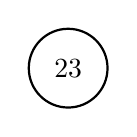
\begin{tikzpicture}[thick]
      \node[circle, draw, minimum size = 1cm]{23};
    \end{tikzpicture}
\end{minipage}\hfill
\begin{minipage}{0.55\textwidth}
    We start with an empty tree, and add our root node: $23$.
\end{minipage}

\begin{minipage}{0.35\textwidth}
    \begin{tikzpicture}[
      node distance = 1.5cm,
      level distance=1.5 cm,
      level 1/.style={sibling distance=3cm},
      level 2/.style={sibling distance=1.5cm},
      thick, minimum size=1cm]
      \node[circle,draw](23) {23}
	    child {
	    node [circle,draw](17){17}
	    }
	    child{node[circle,draw](476){476}
	    };
      \path[->, >=stealth', shorten >=1pt, auto]
	    (23) edge[bend right, blue] (17)
	    (23) edge[bend left, red] (476);
    \end{tikzpicture}
\end{minipage}\hfill
\begin{minipage}{0.55\textwidth}
    Now we add two children: $17$ and $476$.
    Clearly, $17$ becomes the left child because $17 < 23$, and $476$ becomes the right child because $476 > 23$.
\end{minipage}

\begin{minipage}{0.35\textwidth}
    \begin{tikzpicture}[
      node distance = 1.5cm,
      level distance=1.5 cm,
      level 1/.style={sibling distance=3cm},
      level 2/.style={sibling distance=1.5cm},
      thick, minimum size=1cm]
      \node[circle,draw] {23}
	    child {
	    node [circle,draw]{17}
	    }
	    child{node[circle,draw]{476}
		    child{node[circle,draw](28){28}}
		    child[fill=none] {edge from parent[draw=none]}
	    };
      \path[->, >=stealth', shorten >=1pt, auto]
      (23) edge[bend left, red] (476)
      (476) edge [bend right, blue] (28);
    \end{tikzpicture}
\end{minipage}\hfill
\begin{minipage}{0.55\textwidth}
    What happens if we add $28$? Starting at the root, we move to the right because $28 > 23$.
    However, there is already a right subroot there!
    $28$ must then take $476$ as its parent node and, because $28 < 476$, it is placed as the left child of $476$.
\end{minipage}

To begin writing an insertion method for our \li{BinarySearchTree} class, we consider BST's themselves.
BSTs are a recursive data structure because each of the left and right subtrees of a parent node are, themselves, BSTs.
Therefore, many of the algorithms for working with binary search trees can also be recursive.
A recursive function is a function that calls itself until it reaches a base case.
In the case of a BST, the recursive function allows us to travel right or left as appropriate until we reach a missing subtree.
To supplement our \li{insert} method, we will write a recursive function to call within our insert function:
\begin{lstlisting}
def insert(self, data):
    def _recur_insert(node, item):
        # This is the base case; we have reached the proper node for insertion
        # and we now return the data as a Node to the previous function call,
        # setting it as the right or left node of its parent.
        if node is None:
            return Node(item)
        else:
            # Recursively travel through the tree until you reach a leaf node
            if item < node.value:
                node.left = _recur_insert(node.left, item)
            elif item > node.value:
                node.right = _recur_insert(node.right, item)

        # After the base case, each of the previous calls to the
        # recursive function finishes by returning the previous node.
        return node

    self.root = _recur_insert(self.root, data)
    self.size += 1
\end{lstlisting}
We call this recursive function and set it equal to the root node.
The function will continually call itself until it finds an empty node.
It inserts the data as a node, and then \li{return node} will finish each of the previous calls to the recursive function.
(It simply returns each of the parents it recursively visited prior, re-setting them equal to themselves, until it finally returns to \li{self.root}.)
Finally, we finish our insertion method by updating our size.

\subsection*{Searching}
Although recursive functions are often useful and intuitive with trees, we are by no means required to use them.
In fact, for large trees, a recursive algorithm may incur a large overhead.
When writing a method to search for nodes in a BST, we may either use recursion or an alternate method to ascertain whether a piece of data is to be found within the tree.

\begin{problem}
Add a method for finding nodes to your binary tree class. If a node containing your data exists within the tree, return the node.
If no such node exists, return \li{False}.
\label{prob:Finding Nodes}
\end{problem}

\subsection*{Removing}
Removing nodes is only slightly more complicated.
We have three cases to consider:
\begin{enumerate}
\item No children.
This is the most straightforward case.
If the node we want to delete has no children then we simply remove the node.
\begin{center}
\begin{minipage}{0.3\textwidth}
    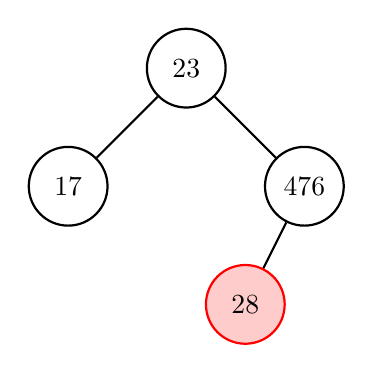
\begin{tikzpicture}[
      level distance=1.5 cm,
      level 1/.style={sibling distance=3cm},
      level 2/.style={sibling distance=1.5cm},
      thick, minimum size=1cm]
      \node[circle,draw](23) {23}
	    child {
	    node [circle,draw](17){17}
	    }
	    child{node[circle,draw](476){476}
	    	child{node[circle,draw=red, fill=red!20!](28){28}}
	    	child[fill=none] {edge from parent[draw=none]}
	    };
    \end{tikzpicture}
\end{minipage}
\begin{minipage}{0.2\textwidth}
   \begin{center}
     \begin{tikzpicture}[]
        \draw[->, double, double equal sign distance, -implies, thick] (0,0) -- (1.25,0);
    \end{tikzpicture}
   \end{center}
\end{minipage}
\begin{minipage}{0.3\textwidth}
    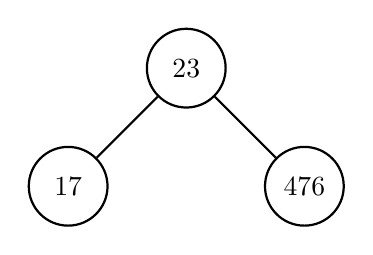
\begin{tikzpicture}[
      level distance=1.5 cm,
      level 1/.style={sibling distance=3cm},
      level 2/.style={sibling distance=1.5cm},
      thick, minimum size=1cm]
      \node[circle,draw](23) {23}
	    child {
	    node [circle,draw](17){17}
	    }
	    child{node[circle,draw](476){476}
	    };
    \end{tikzpicture}
\end{minipage}
\end{center}

\item One child.
In this case, we have to worry about children.
If we were to just delete the node, we would lose the entire subtree.
The solution, however, is simple enough: we promote the single child to take the place of the node we are deleting.
This preserves the binary search property.
\begin{center}
\begin{minipage}{0.3\textwidth}
    \begin{tikzpicture}[
      level distance=1.5 cm,
      level 1/.style={sibling distance=3cm},
      level 2/.style={sibling distance=1.5cm},
      thick, minimum size=1cm]
      \node[circle,draw](23) {23}
	    child {
	    node [circle,draw](17){17}
	    }
	    child{node[circle,draw=red, fill = red!20!](476){476}
	    	child{node[circle,draw](28){28}}
	    	child[fill=none] {edge from parent[draw=none]}
	    };
     \path[->, >=stealth', shorten >=1pt, auto]
      (28) edge[bend left, red] (476);
    \end{tikzpicture}
\end{minipage}
\begin{minipage}{0.2\textwidth}
   \begin{center}
     \begin{tikzpicture}[]
        \draw[->, double, double equal sign distance, -implies, thick] (0,0) -- (1.25,0);
    \end{tikzpicture}
   \end{center}
\end{minipage}
\begin{minipage}{0.3\textwidth}
    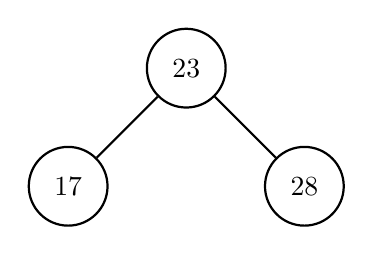
\begin{tikzpicture}[
      level distance=1.5 cm,
      level 1/.style={sibling distance=3cm},
      level 2/.style={sibling distance=1.5cm},
      thick, minimum size=1cm]
      \node[circle,draw](23) {23}
	    child {
	    node [circle,draw](17){17}
	    }
	    child{node[circle,draw](28){28}
	    };
    \end{tikzpicture}
\end{minipage}
\end{center}
\item Two children.
We need to be a little careful in this case.
We can't simply promote a child node.
Indeed, how would we decide which child to promote?
Fortunately, we can reduce this case down to one of the previous two cases.
Suppose we are removing node $23$, which has two children.
We first locate either the smallest node of the right subtree or the greatest node of the left subtree.
In this case, we identify node $28$ as the smallest node in the right subtree.
Because $28$ is the smallest node of the right subtree, it cannot have a child to its left, which implies it either has one child to the right or no children at all.
We swap the data of nodes $28$ and $23$ (so node $28$ now has the data that $23$ had and vice versa).
This swap still preserves the binary search property of the tree and removing $23$ has been reduced to a simpler case.
\begin{minipage}{0.3\textwidth}
\begin{tikzpicture}[
  level distance=1.5 cm,
  level 1/.style={sibling distance=3cm},
  level 2/.style={sibling distance=1.5cm},
  thick, minimum size=1cm]
  \node[circle,draw=red, fill = red!20!](23) {23}
	child {
	node [circle,draw]{17}
	}
	child{node[circle,draw]{476}
		child{node[circle,draw](28){28}}
		child[fill=none] {edge from parent[draw=none]}
	};	
  \path[->, >=stealth', auto]
     (23) edge[out = 5, in=15, blue, looseness=1.5] (28)
     (28) edge[bend left, red] (23);
\end{tikzpicture}
\end{minipage}
\begin{minipage}{0.2\textwidth}
   \begin{center}
     \begin{tikzpicture}[]
        \draw[->, double, double equal sign distance, -implies, thick] (0,0) -- (1.25,0);
    \end{tikzpicture}
   \end{center}
\end{minipage}
\begin{minipage}{0.3\textwidth}
    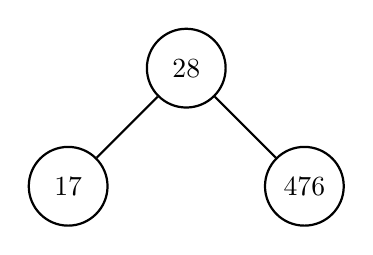
\begin{tikzpicture}[
      level distance=1.5 cm,
      level 1/.style={sibling distance=3cm},
      level 2/.style={sibling distance=1.5cm},
      thick, minimum size=1cm]
      \node[circle,draw](28) {28}
	    child {
	    node [circle,draw](17){17}
	    }
	    child{node[circle,draw](476){476}
	    };
    \end{tikzpicture}
\end{minipage}
\end{enumerate}

\begin{problem}
Provided below is a removal method for binary search trees.
The \li{_recur_remove} method takes two arguments: the parent node, n; and the candidate for removal, cand.
For this problem, edit the following code by inserting comments explaining each step of the removal method.

\begin{lstlisting}
def remove(self, item):
    def _recur_remove(n, cand):
        if n is None:
            return
        else:
            if cand < n.value:
                n.left = _recur_remove(n.left, cand)
            elif cand > n.value:
                n.right = _recur_remove(n.right, cand)
            elif cand == n.value:
                if n.left is None and n.right is None:
                    return
                elif n.left is not None and n.right is None:
                    nleft = n.left
                    del n
                    return nleft
                elif n.left is None and n.right is not None:
                    nright = n.right
                    del n
                    return nright
                else:
                    nmin = n.right
                    while nmin.left is not None:
                        nmin = nmin.left
                    n.value, nmin.value = nmin.value, n.value
                    n.right = _recur_remove(n.right, nmin.value)
                    return n
            return n
    if self.root is None:
        return
    else:
        self.root = _recur_remove(self.root, item)
    self.size -= 1
\end{lstlisting}
\label{prob:Binary Removal}
\end{problem}

If data we put in a binary search tree is ordered, we lose the efficiency advantage of these trees.
We can use a balanced binary search tree to avoid this issue and retain the efficiency of binary search trees for any kind of data.

\section*{Hash Tables}
A \emph{hash table} is a very simple data structure that trades memory space for speed.
The key advantage of a hash table is this speed; most of the operations of a hash table execute very efficiently, independent of its size.
As such, hash tables have very fast lookup times; they form the underlying data structure for Python's set and dictionary types.

One of the key components of a hash table is a \emph{hash function}.
A hash function takes a piece data as an input and outputs a natural number which corresponds to the index for that piece of data.
Since the hash function must be executed to perform any operation on the hash table (e.g. insertion or lookup), it is imperative that the hash function execute quickly.
Thus, the heart of a hash table is a good hash function.

We begin defining our \li{HashTable} class, then, by allocating space within a one-dimensional array (in this case, a Python list) and by taking both the array size and the hash function as arguments.
\begin{lstlisting}
class HashTable(object):
    def __init__(self, capacity):
        # Efficiently extend a list to the designated hash table size
        self.hashtable = [None] * capacity
        # Keeps track of the number of elements within the hash table
        self.size = 0
        # Indicates the size of the hash table
        self.capacity = capacity

    def load_factor(self):
        # The load factor tells how saturated a hash table is
        return float(self.size)/self.capacity
\end{lstlisting}


A good hash function will execute quickly and distribute items uniformly throughout the table.
In the hash tables in this lab, we will use Python's built-in \li{hash} function.
This code demonstrates the principle steps of inserting into a hash function.
Instead of using our \li{HashTable} class, however, we simply use a similar construct to show how the steps might be implemented in a specific instance:
\begin{lstlisting}
>>> capacity = 5
>>> table = [None] * capacity
>>> hash('three')
8354070563160704301
>>> hash('three') % capacity
1
>>> table[1] = 'one'
>>> print table
[None, 'three', None, None, None]
>>> table[hash('four') % capacity] = 'four'
>>> table[hash('five') % capacity] = 'five'
>>> print table
['four', 'three', 'five', None, None]

# We can locate 'five' quickly
# Notice that is faster than the list's builtin methods
>>> %timeit table.index('five')
1000000 loops, best of 3: 190 ns per loops
>>> %timeit table[hash('five') % capacity]
10000000 loops, best of 3: 111 ns per loop
>>> table[hash('two') % capacity] = 'two'
# Note that our load factor is 4/5.
>>> print table
['four', 'three', 'five', 'two', None]

# When our load factor passes a certain threshold, we need to make the hash table bigger
# Resizing the hash table means rehashing everything in it
>>> def resize(table, new_cap):
        new_table = [None] * new_cap
        for i in table:
            new_table[hash(i) % new_cap] = i
        return new_table
>>> table = resize(table, 7)
>>> print table
[None, None, None, 'two', None, None, 'four']
\end{lstlisting}

The ideal hash function maps unique inputs to unique outputs that are uniformly distributed over the hash space.
However, it is extremely difficult to create an ideal hash function; most hash functions will experience hash collisions.
Hash collisions are when two unique inputs are mapped to the same index in the hash table (in our example above, resizing the hash table resulted in hash collisions that lost half the strings we stored in the table).
Fortunately, there are ways to handle hash collisions.

\paragraph{Probing.}
One method that we can use to resolve hash collisions is probing.
A short example will be succintly illustrate this method.
\begin{lstlisting}
>>> capacity = 5
>>> table = [None] * capacity
# Now we add the words 'one' and 'two'
# Notice what happens when we add 'two'
>>> table[hash('one') % capacity] = 'one'
>>> print table
[None, None, None, 'one', None]
>>> table[hash('two') % capacity]
'one'

# We can resolve the collision by looking for the next available index
# Starting at index 3, we look at index 3+1 % capacity, 3+2 % capacity, 3+3 % capacity, ..., until we find and empty index
# Seeing that index 4 is None, we store 'two' there
>>> table[4] = 'two'
>>> print table
[None, None, None, 'one', 'two']
\end{lstlisting}
This is called linear probing.
There are other variations of this idea which are more optimal.

\paragraph{Chaining.}
Another method for resolving hash collisions is chaining.
This method slightly alters the structure of our hash table, so that at each index, a list is stored.
When an item is mapped to an index, it is appeneded to the list at that index.
\begin{lstlisting}
>>> capacity = 5
>>> table = [list() for i in xrange(capacity)]

# Now we add the words 'one' and 'two'
# Notice what happens when we add 'two'
>>> table[hash('one') % capacity].append('one')
>>> print table
[[], [], [], ['one'], []]
>>> table[hash('two') % capacity].append('two')
>>> print table
[[], [], [], ['one', 'two'], []]
\end{lstlisting}

\begin{problem}
Using the concepts illustrated in the examples above, and an insert method to your \li{HashTable} class. 
Don't forget to update your size for the number of elements within the hashtable!
Use chaining to handle hash collisions (namely, implement your insert method via chaining).

Then, create a method for your hash table to resize. 
Implement this method such that, when your hash table exceeds a load factor of $.8$, it will resize the hash table so that the load factor is below $.3$.
Don't forget to rehash the elements already within your table!

Initialize a hash table of size 4 and insert the following felines: `lion', `tiger', `cheetah', `cougar', `colocolo', `cat', `clouded leopard', and `jaguar'.
Print your hash table.
\label{prob:hash_table}
\end{problem}

\begin{info}
Usually exisiting implementations of data structures are better to use.
The implementations of linked lists, trees, and hash tables in this lab were designed to familiarize you with the data structure's mechanics through example and practice.
In real situations, you will likely use Python's deques, sets, or dictionaries.
Python doesn't have a built-in implementation of trees, but there are several Python libraries that have highly optimized implementations of trees.

Performance tuning for data structures can be tricky even for professionals.
For this reason, it is better to avoid writing your implementation when one already exists.
\end{info}
